\documentclass[a4paper]{article}

%% Language and font encodings
\usepackage[
    	backend=biber,
    	bibstyle=ieee
	]{biblatex} %ydnt: Sort by year (descending), name, title.
    \addbibresource{biblio.bib}
    
\usepackage[utf8]{inputenc}

%% Sets page size and margins
\usepackage[a4paper,top=3cm,bottom=2cm,left=3cm,right=3cm,marginparwidth=1.75cm]{geometry}

%% Useful packages
\usepackage{amsmath}
\usepackage{graphicx}

\usepackage[colorinlistoftodos]{todonotes}
\usepackage[colorlinks=true, allcolors=blue]{hyperref}

\usepackage{geometry}
    \geometry{left=2cm}
    \geometry{right=2cm}
    \geometry{top=2cm}
    \geometry{bottom=2cm}
    
%\renewcommand\bibname{References}
	
	\usepackage{etoolbox}
	\makeatletter
	\patchcmd{\chapter}{\if@openright\cleardoublepage\else\clearpage\fi}{}{}{}
	\makeatother%to suppress newpages on chapters

%Formatting titles
    \usepackage{titlesec}
 
\titleformat{\chapter}
    {\Large\bfseries}
    {\thechapter}
    {8pt}{}   
\titlespacing*{\chapter}{0pt}{-\topskip}{15pt}%left-before-after, topskip for less space before new chapter

\titleformat{\section}
    {\large\bfseries}
    {\thesection}
    {1em}{}
\titlespacing*{\section}{0pt}{8pt}{20pt}
 
\titleformat{\subsection}
    {\normalsize\bfseries}
    {\thesubsection}
    {1em}{}
    
%%%%%%%%%%%%%%%%%%%%%%%%%%%%%%%%%%%%%%%%%%</PREAMB>%%%%%%%%%%%%    
    
\title{Key Words Extraction from News}
\author{Aleksandr Safin, Ivan Rodin, Maxim Kaledin}

\begin{document}
\maketitle
\begin{abstract}
In this project several techniques are proposed for keywords extraction problem from news. News stories is a very special type of data: they are typically small texts with lots of named entities and there is no much data for supervised methods. In this project we propose methods based on Latent Semantic Analysis, topic modelling, different graph methods using Graph of Words representation of text. The methods are tested on 500KN-Crowd dataset, most of them do not require training dataset, have simple architecture and show very reasonable results during manual and automatic testing.
\end{abstract}
\section*{Introduction}

The keywords is a well-known problem in linguistics and natural language processing which has a huge variety of applications. People can use keywords to decide whether the text is relevant, briefly catch the main idea. Machines can use them in recommender system (to recommend you goods based on the reading history), search engines (document indexing).

News stories is a very specific type of texts. They are relatively small (usually no more than 600-700 words) and have a large number of named entities (people, places, organizations,...). Moreover, there is no much (freeware) data for statistics approaches to operate effectively. Here we can propose other unsupervised methods to roughly estimate keywords. The challenge is to use as few number of input texts as possible (usually, only one) and produce results very fast.

The problem of keywords can be solved using modern machine learning approaches and statistical methods. Our goal is to investigate other class of approaches, i.e. heuristic methods arising from graph clustering (known as community detection in social network analysis), random walk models (TextRank) and methods of topic modeling. All code and relevant documents can be found on project's Github \cite{our:Github}.

\section*{Problem statement}

Input texts usually are relatively small (up to 600-700 words), we should produce the \textit{keywords} based on it. The \textit{keywords} are the most important words which could help to roughly estimate the gist of text without reading it. In different approaches the set of keywords is defined differently.

\subsection*{Quality Estimation}

We use Jaccard index and 500KN-Crowd dataset \cite{Marujo:LREC:2012} with manually extracted keywords to roughly measure the quality of prediction:

$$
K_J = \frac{\vert A \cap B \vert}{\vert A \cup B\vert},
$$

where $A$ is set of extracted keywords $B$ are gold standard keywords. But since our test data has about 30-40 keywords on each text, this metrics may be very bad, however the keywords turns out to be reasonable. So we also consider average number of guessed words (in comparison with gold standard) as another quality measure. 

\section*{Matrix factorization-based approach (A. Safin)}

\subsection*{Approximation}

Of course, one could propose simple baseline, like consider TF-IDF document-term matrix and then choose the words  corresponding to the top highest scores. But the question is could we do better.   

Since keywords of the document reflect essential part of the whole document, then we simply consider here that the task of keywords extraction from the documents could be formulated as  the task of finding low-rank approximation of the term-document matrix. 

Then, to extract keywords for each document simply means to choose $k$ (for instance) words (or bigrams, if they are used it the bag of words vector) corresponding to the highest values in the approximated matrix.

So, the task could be formally described as:
$$
\underset{\text{rank}A_r = r}{\text{minimize }} \|A - A_{r}\|_{F}^2,
$$
where the $r$ is the parameter of the model which could be optimized to provide acceptable results for key word extraction.

One approach to obtain such approximation is to use SVD  and then truncate it up to $r$ largest singular values \cite{LSAfounds}.

Another approach utilizes the following idea, that term-document matrix (probabilities of each word to be in the particular document) could be represented is a product of two matrices such that $p(w_i | d_j) = \sum_{k=1} p(w_i | t_k)p(t_k | d_j)$. In other words, one could consider the initial term-document matrix $A$ as $A=FH$, where $F$ is matrix determined by $p(w_i|t_k)$ and $H_{kj} = p(t_k | d_j)$. So, the most weighted elements in the $j^{th}$ column of the matrix $F$ reflects the keywords for the $j^{th}$ topic. And matrix $H$ reflects the probability of each topic for every document. Because we want consider the elements of $H$ and $F$ matrices as a probabilities (or proxy values for probabilities), it is natural to require that $F$ and $H$ would be non-negative.

The task of Non-negative Matrix Factorization \cite{NMF:topics} (NMF) could be formalized as:
$$
\underset{F \geq 0, H \geq 0}{\text{minimize }} \|A - FH\|_{F}^2
$$

\subsection*{Keywords extraction}

So, to extract keywords based on NMF or SVD approximation for the whole set of documents we simply choose the words corresponding to the highest scores.

But there could be a pretty simple modification. Let us construct the TF-IDF matrix for each document, namely treating each sentence as document. So, what we obtain is TF-IDF sentence-term matrix. Then after matrix factorization, we choose the words corresponding to the highest scores in the first row of the matrix which reflects topic-word relations.

In the SVD-based factorization this means that we choose the most important topic among all sentences.


Another approach to extract keywords is to utilize the LSA approach, namely using NMF for finding the set of most appropriate keywords for the topics seemed to be in the document (according to NMF). And then select appropriate keywords which are relevant to the document.

\subsection*{PageRank for the graph of words}
The idea is to find PageRank for the graph of words and it was proposed in \cite{Mihalcea04TextRank} and is referred to as TextRank. Consider a graph $G = (V, E)$ of words, namely $V$ is the set of words and the weight of the edge $e_{ij}$ equals to the number of cases when the word $j$ occurs after the word $i$ within the window of the fixed size $w_{size}$. Thus, we assign to each word a score corresponding to the PageRank score. Then, we just output the words with the highest PageRank score.

The Table \ref{table:timeres} shows that TextRank works more slower than matrix factorization methods. This is simply because of the a lot of preprocessing of natural language text and construction of the graph of words.

\begin{center}
\begin{figure}[h!]
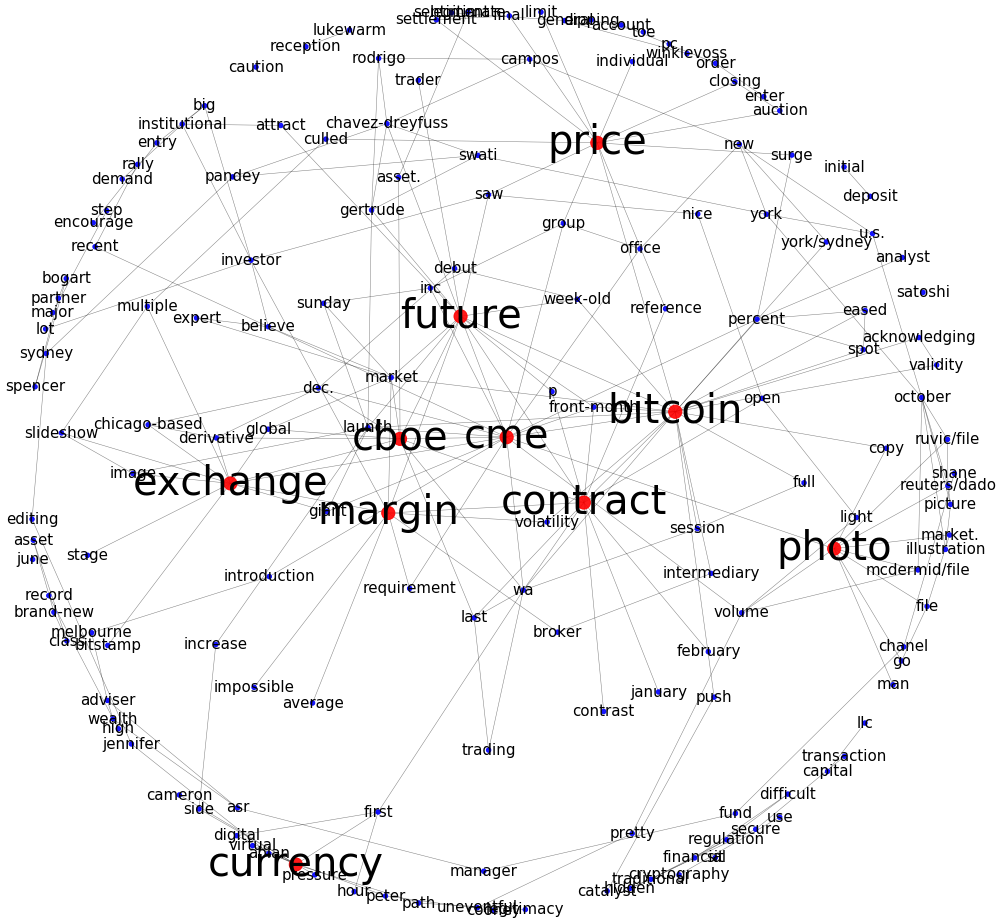
\includegraphics[scale=1]{textrank_example.png}
\caption{Reuters news \href{https://uk.reuters.com/article/us-bitcoin-futures/exchange-giant-cmes-bitcoin-futures-get-tepid-take-up-in-debut-idUKKBN1EB04N}{story}, "Bitcoin hits bigger stage as exchange giant CME launches futures", TextRank-based keywords}
\end{figure}
\end{center}

    \begin{table}[h!]
      \center
      \begin{tabular}{|p{3cm}|p{14cm}|}
      \hline
      Approach & Keywords \\
      \hline
      SVD-based & 'nakamoto' 'use' 'secure' 'satoshi' 'cryptography' 'regulation' 'traditional' 'transactions' 'successfully' 'making' \\
      \hline
      NMF-based & '19' 'contract' 'price' 'reference' 'set' '18' '805' 'january' 'sponsored' 'exchange' \\
      \hline
      TextRank & 'bitcoin' 'cme' 'future' 'contract' 'exchange' 'price' 'photo' 'margin' 'cboe' 'currency' \\
      \hline
      \end{tabular}
      \caption{Comparison of results for different approaches}
    \end{table}


    \begin{table}[h!]
        \center
        \begin{tabular}{|p{3cm}|p{2cm}|}
        \hline
        Approach & Average time (secs / text)  \\
        \hline
        SVD-based & 0.0047 \\
        \hline
        NMF-based & 0.0237 \\
        \hline
        TextRank & 0.418 \\
        \hline
        \end{tabular}
        \caption{Time performance comparison of the approaches}
        \label{table:timeres}
	\end{table}


%%%%%%%%%%%%%%%%%%%%%%%%%%%%%%%%%%%%%%%%%%%%%%%%%%%%%%%%%%%%%%%
\clearpage

\section*{Extracting Keywords using Optimization of Modularity(M. Kaledin)}

Let $G=(V,E)$ be a graph of words which is built from raw text, where $V$ is a set of words (we leave only nouns and adjectives from original text). Two vertices $u,v$ are connected if $u$ is followed by $v$ in the text within sliding window $w$, this graph can be directed (used for pageRank in this project) or undirected, I consider the latter case. Here is a brief example.

Our aim is to effectively cluster this graph (in social network analysis this process is called \textit{community detection}), then assign keywords by choosing the largest cluster.

\subsection*{Modularity Approaches}


The first algorithm suggesting to use modularity was Girvan-Newman's  algorithm \cite{Girvan:11062002}. It suggests to optimize the \textit{modularity} $Q$ of partition of the graph $G=(V,E)$, $\vert V \vert = n$, $\vert E \vert = m$. Suppose, we search the best graph partition into two communities (subgraphs with large density inside and less outside edges), let $s_i=1$ if vertex $i$ belongs to cluster $1$ and $-1$ otherwise. The article suggests to consider the difference between the actual number of edges between two vertices and the expected one if they were randomly generated with uniform distribution. Thus
$$
Q = \sum_{u,v \in V: ~u \neq v }\left( A_{ij}-\frac{k_uk_v}{2m}\right)\left(s_is_j+1\right) 
$$
defines the modularity of partition. It was noted that this approach can be generalized on case of several communities \cite{Newman:LargeNetworks} with
$$
Q=\sum_{u,v \in V: ~u \neq v }\left( A_{ij}-\frac{k_uk_v}{2m}\right)\delta(c_u,c_v), 
$$
where $c_u,c_v$ denote community assignments and
$$
\delta(c_u,c_v)=
  \begin{cases}
            0 & \text{if $c_u=c_v$} \\
            1 & \text{otherwise} 
  \end{cases}.
$$
Also it is possible to use the hierarchical approach with 2-community clustering \cite{Newman:Structure}. This can be solved as LP with $O(n^3)$ transitivity constraints:
\begin{align*}
& \max_{\delta_{uv}} Q, s.t.\\
& \delta_{uv} + \delta_{vw} \leq 2 \delta_{uw} ~ \forall u,v,w \in V,
\end{align*}
which is very hard even if $n \sim 10^2$. Thus direct optimization of modularity is exhausting (NP-hard with ILP, or worse with quadratic IP), so several sub-optimal algorithms are suggested.

\subsubsection*{Girvan-Newman Algorithm}

Algorithm make useof \textit{betweeness centrality} of edge in a graph: it is a number of shortest paths which include this edge. The idea is that the most "betweeness" edges connect communities. Algorithm sequentially delete the most central edge and recalculates centralities until no edges \cite{Girvan:11062002}. This method is implemented in NetworkX.

\subsubsection*{Louvain Method}

This is quite effective heuristic algorithm for community detection proposed in \cite{Blondel:Louvaine}. On first step all vertices are assigned to its own community, then iteratively we try to reassign each vertex to its neighbouring community. The community of choice is such that it gives the largest increase of modularity. The second step repeats the first step but each node is a detected community and two communities are connected if they have edges connecting them. This method is implemented in python-louvain library as best\_partition.

\subsection*{Other Heuristic Approaches}
\subsection*{Fluid-Based Technique for Community Detection}

I briefly describe also another heuristic algorithm proposed in \cite{Pares:Fluid}. It chooses the number of community fluids $k$ (in our framework I choose it to get maximum modularity), place their start points in random vertices, then run the fluids. Each vertex updates its community with respect to update rule. Denote by $d(c)=1/ \vert c \vert$ the density of community $c$. Compute

\begin{align*}
	C_v = \text{Argmax}_{c} \sum_{w \in v,\Gamma(v)} d(c)\delta (c(w),c) ,
\end{align*}
	where $c(w)$ is a community assigned to vertex $w$, $\Gamma (w)$ is the set of neighbours of $v$. If $C_v$ contains the original community, $v$ stays there, otherwise the new community is chosen among found with uniform distribution. The process is bounded by max\_iterations parameter.\\

This algorithm is implemented in NetworkX library and considered only for comparison with other methods. Unfortunately, it does not work with disjoint graphs, so it is not chosen for the quality estimation. Moreover, it turned out to be very ineffective method on manual experimets.

\subsection*{K-core Technique for Community Detection}

Consider also $k$-core approach for clustering. The maximal subgraph of $G$ of vertices of minimum degree $k$ is called a \textit{$k$-core} \cite{Peng:KCore}. The $k$-core corresponding to the largest possible $k$ is called the \textit{main core}. In this approach we should assign keywords as the main core.

\subsection*{Keywords Extraction}
Let $w$ denotes window size. Firstly, I tokenize the input text with default tokenizer from NLTK framework. Then simple preprocessing goes:
\begin{itemize}
\item Removing punctuation;
\item POS-filtering to leave only nouns and adjectives (supplied by NLTK framework);
\item Removing stop-words (if any, supplied by NLTK);
\item Creating a dictionary from the filtered text, output it and text without punctuation.
\end{itemize}
Then undirected graph of words is built with window size $w$ ($3$, by default). After this I apply $k$-core decomposition to extract the most dense subgraph (known approach, maximal subgraph with all vertices having degree at least $k$ is called a \textit{k-core}, the $k$-core corresponding to the largest $k$ is called the \textit{main} core). This is done becuse the original graph is very sparse and there are many non-relevant words.\\

Then we apply community detection algorithm to extract communities and assign keywords as the largest community.

\subsubsection*{Example of the Keywords extracted}

Consider the example with Reuters news \href{https://uk.reuters.com/article/us-bitcoin-futures/exchange-giant-cmes-bitcoin-futures-get-tepid-take-up-in-debut-idUKKBN1EB04N}{story}, "Bitcoin hits bigger stage as exchange giant CME launches futures". We have already seen its graph of words for windows size equals 2, here are the community plots. I had to set window size to $5$ for fluid algorithm because it does not work with disjoint graphs.

\begin{table}[h!]
\center
\begin{tabular}{|p{3cm}|p{14cm}|}
\hline
Approach & Keywords \\
\hline
Louvain & 'average' 'bitcoin' 'brokers' 'contract' 'contracts' 'contrast' 'experts'
 'february' 'front' 'full' 'futures' 'intermediaries' 'january' 'last'
 'launch' 'march' 'margin' 'market' 'month' 'old' 'p' 'refers'
 'requirement' 'requirements' 'session' 'sunday' 'trader' 'trading'
 'validity' 'volatility' 'week' \\
 \hline
Girvan-Newman & 'validity' 'analysts' 'volatility' 'debut' 'week' 'bigger' 'bitcoin'
 'session' 'intermediaries' 'old' 'brokers' 'spot' 'stage' 'launch'
 'sunday' 'percent' 'full' 'contracts'\\
 \hline
Fluid & 'reception' 'analysts' 'reference' 'regulation' 'requirement' 'average'
 'big' 'bitstamp' 'secure' 'settlement' 'brokers' 'side' 'step' 'surge'
 'trader' 'contract' 'traditional' 'contrast' 'transactions' 'cryptography'
 'volatility' 'demand' 'difficult' 'digital' 'entry' 'exchanges' 'february'
 'final' 'financial' 'first' 'half' 'hidden' 'higher' 'hour' 'impossible'
 'institutional' 'intermediaries' 'investors' 'january' 'last' 'launch'
 'light' 'limits' 'lot' 'lukewarm' 'major' 'march' 'margin' 'multiple'
 'nice' 'open' 'p' 'percent' 'pressure' 'price'\\
 \hline
KCore & 'global' 'reuters' 'rodrigo' 'bitcoin' 'brendan' 'swati' 'campos' 'cboe'
 'chavez' 'sydney' 'cme' 'contract' 'dado' 'u' 'margin' 'market' 'markets'
 'mcdermid' 'volume' 'min' 'month' 'york' 'new' 'dreyfuss' 'october'
 'exchange' 'pandey' 'file' 'front' 'photo' 'read' 'futures' 'ruvic'
 'gertrude'  \\
 \hline
\end{tabular}
\caption{Comparison of results for different approaches: we can see that the keywords are relevant for all methods except fluid algorithm}
\end{table}

\clearpage


The following table and charts show the quality estimates of the algorithms.

\begin{table}[h!]
\center
\begin{tabular}{|l|c|r|}
\hline
Approach & Jaccard's Index & Average number of guessed keywords \\
\hline
Louvain & 0.0702 & 4.01333333333\\
 \hline
Girvan-Newman & 0.0694 & 3.94444444444\\
 \hline
KCore & 0.0948 & 6.5444\\
 \hline
\end{tabular}
\caption{Comparison of quality measures for different approaches}
\end{table}



\clearpage

%%%%%%%%%%%%%%%%%%%%%%%%%%%%%%%%%%%%%%%%%%%%%%%%%%%%%%%%%%%%%%%%%%%%%%%%%%%%%%
\section*{EM algorithm (I. Rodin)}

For finding Non-negative Matrix factorization for initial term-document matrix $A$ one can apply EM algorithm.

Let $W$ be a dictionary of all words, $D$ is a collection of documents, and $n_{dw}$ be a frequency of word $w$ in document $d$. Then we want to find model $p(w|d) = \sum_{t\in T}f_{wt}H_{td}$ with parameters $F_{W\times T}$ and $H_{T\times D}$:

$f_{wt} = p(w|t)$ - probability of word $w$ in topic $t$

$h_{td} = p(t|d)$ - probability of topic $t$ in document $d$.

Then we have the following optimization task for maximization of log-likelihood:

$$\begin{cases}
\sum_{d\in D}\sum_{w\in W}n_{dw}\ln\sum_{t\in T}f_{wt}h_{td} \rightarrow \max\\

s.t.\\

f_{wt}\geq 0, h_{td}\geq 0\\

\sum_wf_{wt} = 1, \sum_th_{td} = 1
\end{cases}$$

This optimization task can be solved by EM algorithm. EM algorithm is a method of simple iterations constisting of 2 steps:

E-step:

$p_{tdw} = norm_{t}(f_{wt}h_{td})$

M-step:

$f_{wt} = norm_{w}(n_{wt})$, $n_{wt} = \sum_dn_{dw}p_{tdw}$

$f_{td} = norm_t(n_{td})$, $n_{td} = \sum_wn_{dw}p_{tdw}$

where $norm_{i\in I}(x_i) = \frac{max(x_i, 0)}{\sum_{j\in I}max(x_j,0)}$

The main advantage of EM algorithm is that it allows implementation of regularizators for tuning the model and adding sparsity to matrices $F$ and $H$.

Sparsity of these matrices means that:

\begin{enumerate}
\item topics are consisting of small number of words, and words from different topics should not intersect a lot (sparsity of matrix $F$);
\item each document should correspond to small number of topics (sparsity of matrix $H$).
\end{enumerate}

For the purpose of finding keywords we would like not to sparse, but smooth matrices, or, in other words, making them more dense.

We will find matrix factorization by means of BigARTM library \cite{vorontsov2014additive}.

After finding dense matrices $F$ and $H$, we will implement the following approach:

\begin{enumerate}
\item For document $d_i$ find topic $t_{j*}$ such that $h_{j*, i}\geq h_{j, i}$
\item Find top $k$ words for topic $j*$ from matrix $F$. These words are considered as keywords of document $d_i$.
\end{enumerate}

\section*{Core-shell cluster (I. Rodin)}

Now let us formulate the following problem:

Let $G = (V, E)$ be a graph of words built from raw text, $V$ is a set of words and two vertices $i$ and $j$ are connected if these words occurs together in sliding window. Let this graph be weighted, and the weight of edge $e_{ij} = e_{ji}$ equals to the number of co-occurence of words $i, j$ withing sliding window in the whole text.The graph is defined by adjacency matrix $A$.

Then we want to find a core-shell cluster $U$ consisting of two non-overlapping parts $U = S \cup R$, where $S$ is a shell of the cluster with average connection rate $\lambda \geq 0$,
and $R$ is a core of the cluster with average connection rate $\lambda + \mu$, where $\mu\geq0$.

In this cluster $R$ is a set of the most strongly-connected words which may be considered as keywords of the text, then $S$ may be considered as a set of ``supporting'' keywords.

Optimization task for extraxting such clusters mey be formulated as follows:

$$\begin{cases}
\sum_{i,j}^N \Big( A_ij - \lambda s_is_j - (\lambda + \mu)r_ir_j \Big)^2 \min\\

s.t.\\

\lambda \geq 0, \mu \geq 0\\

s_i = \{0,1\}, r_i = \{0,1\}, i=1,..,N
\end{cases}$$

Or, in other words, we want to find the approximation for matrix $A$:

$$A = S + R$$

where $S_{ij} = \lambda$ if $s_i, s_j$ are shell elements, and $r_{ij} = \lambda + \mu$ if $r_i, r_j$ are core elements.

The heuristic algorithm for finding sub-optimal solution of this problem is presented in \cite{rodin2017supercluster}.


\section*{Spectral clustering}

Spectral clustering approach uses the eigenvalue of the adjacency or Laplacian matrix of the graph to apply dimension reduction before clustering in fewer dimensions. It refers to a set of heuristic algorithms, all based on idea of computing the first few singular vectors and then clustering in a low dimensional subspace.

In our implementation we have used library sklearn.cluster.SpectralClustering. It turned out that Spectral clustering approach performs quite good in term of guessed keywords -- it has recovered 6.13 words in average, which gives this algorithm second place among all methods.

\newpage

\section*{Results}

Here is a table of all achieved results.

 \begin{table}[h!]
        \center
        \begin{tabular}{|p{3cm}|p{3cm}|p{2cm}|}
        \hline
        Approach & Average Matches & Jaccard Index \\
        \hline
        SVD-based & 3.35 & 0.069\\
        \hline
        NMF-based & 3.59 & 0.076 \\
        \hline
        TextRank & 3.395 & 0.125 \\
        \hline
		Louvain &  4.0133 & 0.0702 \\
 		\hline
		Girvan-Newman &  3.9444 &  0.0694 \\
 		\hline
		KCore &  6.5444 & 0.0948 \\
         \hline
        EM &  4.15 & 0.05 \\
         \hline
        EM regularised &  4.475 & 0.054 \\
         \hline
        Core-shell &  0.96 & 0.023 \\
         \hline
        Spectral &  6.131 & 0.073 \\
         \hline
        \end{tabular}
        \caption{Comparison of the results for different approaches}
     \end{table}
 
\section*{Conclusion}
	In this project we have applied several approaches to the problem of automatic keyword extraction from news. Note that those methods are not very accurate but can be used for rough approximations of keywords. The main advantage of these algorithms is their simplicity. Each algorithm runs relatively fast with one news story given as input and most of them do not require training datasets (except LSA and topic modeling approaches). The proposed algorithms might be useful in recommender systems and estimation of text relevance (search engines, newspaper generation etc.). 

\printbibliography
\end{document}
